% Explicar en que consitió el trabajo (brevemente).
	% - Explicar levemente los criterios usados para la paralelización
	% - Por qué es buena idea usar este tipo de procesamiento en filtros de imágenes. (todos los pixeles reciben exactamente el mismo procesamiento y así en una sola ráfaga se peude levantar y procesar muchos).
	% - Explicar la hipótesis (debería ser n veces mas rápido porque zarasa).
	% - Se intentó estudiar si vale la pena o no el esfuerzo adicional de desarrollo y debuggeo.


	A lo largo de este documento se realizará un análisis consiso sobre el
procesamiento de datos SIMD mediante las intrucciones SSE de la arquitectura
AMD-64. El mismo se hará mediante la comparación de diversas implementaciones
de 3 filtros (2 de video y uno de imágen).

	El procesamiento SIMD consiste en realizar una misma operación sobre varios
datos de manera simultánea. Es decir que lo que se logra es paralelismo a nivel
de datos. Esta clase procesamiento es ideal para realizar filtros sobre imágenes
, porque ahí justamente lo que uno busca es que cada pixel reciba el mismo proceso.


\begin{figure}[h]
\begin{center}
  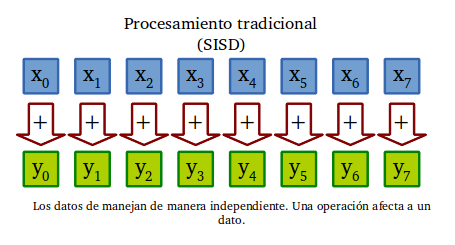
\includegraphics[scale=0.4]{secciones/introduccion/imagenes/SISD.png}
    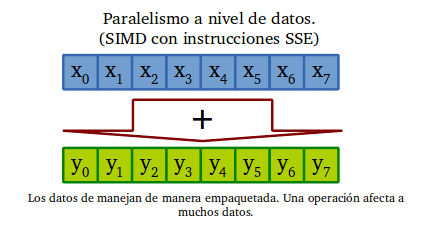
\includegraphics[scale=0.4]{secciones/introduccion/imagenes/SIMD.png}
\end{center}
\caption{Esquemas de procesamiento SISD y SIMD}
\label{fig:SISD-SIMD}
\end{figure}


	Sin embargo para realizar este análisis es imperioso meterse un poco mas adentro.
El comportamiento esperado a priori para estos procesos es una relación inversa entre
el nivel de paralelismo y el tiempo consumido. Es decir, al procesar 4 datos a la vez
uno esperaría obtener que el proceso tarde 4 veces menos tiempo, procesando 8 datos
a la vez 8 veces menos tiempo, etc. Sin embargo esto no siempre ocurre. Durante
este trabajo constantemente se va a intentar explicar que desviaciones se 
produjeron con respecto a este supuesto. Para eso vamos a analizar la arquitectura
intel-64, la velocidad de acceso a memoria, el modo en que se usa la caché,
el medio en el cuál se ejecutan los programas y los algoritmos utilizados entre
otras cosas.

	A lo largo del trabajo se va a ir mostrando como el uso de código de ensamblador
optimizado para el uso de la tecnología SSE produce programas sumamente eficientes. Sin embargo
producir ese código es sumamente trabajoso, mucho mas que usar lenguajes de mas alto nivel como
c o c++. Por ese motivo se intentará hacer otro análisis (tal vez algo menos científico
pero intentando justificar de la manera mas objetiva posible) de cuando vale la pena y cuando no.





	
